\documentclass[14pt]{extarticle}
\usepackage{fontspec}
\usepackage{polyglossia}
\usepackage{amsmath}
\usepackage{amssymb}
\usepackage{xcolor}
\usepackage{fancyhdr}
\usepackage{graphicx}
\usepackage{listings}
\usepackage[most]{tcolorbox}
% \usepackage{setspace}
\usepackage{pifont}
\usepackage{enumitem}
\usepackage{titlesec}
\usepackage[bottom]{footmisc}
\usepackage{titling}
\usepackage{minted}
\usepackage{etoolbox}
\usepackage{array}
\usepackage{extsizes}
\usepackage{float}
\usepackage{booktabs}
\usepackage{hyperref}
\usepackage[onehalfspacing]{setspace}
\usepackage[a4paper, top=2.7cm, bottom=2.7cm, left=2.5cm, right=2.5cm, headheight=1.5cm, headsep=0.5cm]{geometry}
\usepackage{tikz}

\usetikzlibrary{automata, positioning, arrows.meta, arrows}

\newfontfamily\emoji{Segoe UI Emoji}

\pagestyle{fancy}

\setmainlanguage[numerals=western]{arabic}
\setotherlanguage{english}
% \newfontfamily\arabicfont[Script=Arabic]{Amiri}
\newfontfamily\arabicfont[Script=Arabic]{Calibri}
\newfontfamily\arabicfonttt[Script=Arabic]{Courier New}

\lstset{
  language=[Sharp]C,
  numbers=left,
  stepnumber=1,
  numbersep=8pt,
  frame=single,
  basicstyle=\ttfamily\small,
  keywordstyle=\color{blue},
  stringstyle=\color{red},
  commentstyle=\color{green!50!black}
}

\newif\ifdetailed
\ifdefined\setdetailed
  \setdetailed
\fi

\newif\ifwithsols
\ifdefined\setwithsols
  \setwithsols
\fi

% unified tcolorboxes for articles
\tcbset{colback=white, colframe=black, fonttitle=\bfseries, boxrule=0.8pt}
\newtcolorbox{boxDef}[1][]{colback=blue!5!white,colframe=blue!75!black,
  title={{\emoji📘} تعريف\ifx\\#1\\\else ~#1\fi :}}
\newtcolorbox{boxExercise}[1][]{colback=cyan!5!white,colframe=cyan!70!black,
  title={{\emoji🧩} تمرين\ifx\\#1\\\else ~#1\fi :}}
\newtcolorbox{boxExample}[1][]{colback=yellow!5!white,colframe=orange!90!black,
  title={{\emoji📝} مثال\ifx\\#1\\\else ~#1\fi :}}
\newtcolorbox{boxNote}[1][]{colback=gray!10!white,colframe=black,
  title={{\emoji✨} ملاحظة\ifx\\#1\\\else ~#1\fi :}}
\newtcolorbox{boxAttention}[1][]{colback=magenta!10!white,colframe=magenta!80!black,
  title={{\emoji🔔} تنبيه\ifx\\#1\\\else ~#1\fi :}}
\newtcolorbox{boxWarning}[1][]{colback=red!5!white,colframe=red!75!black,
  title={{\emoji⚡} ملاحظة هامة\ifx\\#1\\\else ~#1\fi :}}
\newtcolorbox{boxSolution}[1][]{colback=green!5!white,colframe=green!60!black,
  title={{\emoji✅} حل\ifx\\#1\\\else ~#1\fi :}}
\newtcolorbox{boxSymbol}[1][]{colback=purple!5!white,colframe=purple!70!black,
  title={{\emoji🔣} رمز\ifx\\#1\\\else ~#1\fi :}}
\newtcolorbox{boxHint}[1][]{colback=teal!5!white,colframe=teal!60!black,
  title={{\emoji💡} تلميح\ifx\\#1\\\else ~#1\fi :}}


\tcbset{simplecode/.style={ colback=gray!5, colframe=black!50, boxrule=0.4pt, arc=2pt, left=4pt,right=4pt,top=4pt,bottom=4pt}}
\newenvironment{boxCode}{\begin{tcolorbox}[simplecode]}{\end{tcolorbox}}

\newcolumntype{C}[1]{>{\centering\arraybackslash}p{#1}}

% redefine spaces after titles
\makeatletter
\renewcommand{\@maketitle}{%
  \begin{center}
    {\huge \bfseries \@title \par}%
    \vskip 0.2em % space between title and author
    {\large \@author \par}%
    % \vskip 0.2em % space between author and date
    % {\normalsize \@date \par}%
  \end{center}
}
\makeatother

\fancyhf{} % clear default
\fancypagestyle{plain}{
  \fancyhf{}
  \fancyhead[L]{مدرسة التسامح الشاملة}
  % \fancyhead[L]{
\includegraphics[height=1cm]{../../../images/logoTasamoh.png}}
  \fancyhead[R]{الأستاذ محمود اغبارية}
  \fancyfoot[C]{\thepage}
}

\fancyhead[L]{مدرسة التسامح الشاملة}
\fancyhead[R]{الأستاذ محمود اغبارية}
\fancyfoot[C]{\thepage}
% \date{\today}

\setcounter{tocdepth}{3} % only section subsection and subsubsection in TOC

\newcommand{\importpdfpage}[2]{%
    \thispagestyle{empty}
    \newgeometry{left=0cm,right=0cm,top=0cm,bottom=0cm}
    \includegraphics[page=#2,width=0.95\paperwidth,height=0.95\paperheight,keepaspectratio]{#1}
    \restoregeometry
}

\newcommand{\insertFullImg}[1]{%
    \noindent
    \makebox[\textwidth][c]{
        \includegraphics[width=0.9\paperwidth,keepaspectratio]{#1}%
    }%
}%

% ----------------------


% \begin{document}

% \maketitle

% % \clearpage  % start TOC on a new page
% % \renewcommand{\contentsname}{جدول المحتويات}
% % \tableofcontents
% % \clearpage

% \part*{part 1} % the * prevents numbering
% \section*{مقدمة}
% \subsection*{مثال رياضي}
% \subsubsection*{مثال فرعي}
% \paragraph*{ paragraph 1}
% \subparagraph*{sub paragraph 1}

% \ifdetailed
% \begin{english}
% \begin{minted}{csharp}
% // C# Example
% \end{minted}
% \end{english}
% \fi

% OLD WAY
% \ifdetailed
% \begin{english}
% \begin{lstlisting}
% // C# Example
% \end{lstlisting}
% \end{english}
% \fi

% % 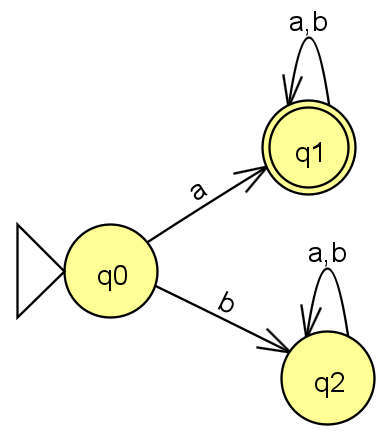
\includegraphics[width=0.2\textwidth]{../../../images/DFAs/ex1_q1.png}



% \vspace{3cm}
% \begin{flushleft}
% أرجو لكم وقتًا ممتعًا.

% الأستاذ محمود اغبارية.
% \end{flushleft}


% \end{document}


\title{ملخّص الدرس: الفئات والكائنات في \textenglish{C\#}}

\begin{document}

\maketitle
\thispagestyle{fancy}

%=============================================================
\section{تعريف الفئة وإنشاء كائن}
%=============================================================

\textbf{الفئة} (\textenglish{class}) هي قالب يصف مجموعة من الخصائص.
\textbf{الكائن} (\textenglish{object}) هو نسخة حقيقية تُنشأ من هذا القالب.

\begin{boxExample}
\begin{english}
\begin{minted}{csharp}
class Book
{
    public string Title;
    public string Author;
    public int Year;
    public double Price;
}
\end{minted}
\end{english}
\end{boxExample}

لإنشاء كائن والوصول إلى خصائصه:

\begin{boxExample}
\begin{english}
\begin{minted}{csharp}
Book b = new Book();
b.Title = "Algebra";
b.Author = "Teacher";
\end{minted}
\end{english}
\end{boxExample}

\begin{itemize}[itemsep=1pt]
    \item الكلمة \textenglish{new} تُنشئ كائنًا جديدًا في الذاكرة.
    \item يمكن إنشاء عدد غير محدود من الكائنات من نفس الفئة، كل منها مستقل عن الآخر.
\end{itemize}

\clearpage
%=============================================================
\section{العمليات الداخلية بدون معاملات}
%=============================================================

\textbf{العملية الداخلية} (\textenglish{method}) هي دالة تُعرَّف داخل الفئة وتعمل على بيانات الكائن مباشرةً، دون الحاجة إلى تمرير الكائن كمعامل.

\begin{boxExample}
\begin{english}
\begin{minted}{csharp}
class Book
{
    // ...
    public void Print()
    {
        Console.WriteLine($"{Author}: {Title} ({Year})");
    }
}
\end{minted}
\end{english}
\end{boxExample}

الاستدعاء من \textenglish{Main}:

\begin{boxExample}
\begin{english}
\begin{minted}{csharp}
// In Main
b1.Print();
\end{minted}
\end{english}
\end{boxExample}

\begin{itemize}[itemsep=1pt]
    \item داخل العملية، يمكن الوصول مباشرةً لجميع خصائص الكائن (\textenglish{Title, Author, ...}) دون الحاجة لكتابة اسم الكائن.
    \item مقارنةً بالعملية الخارجية (\textenglish{static}) التي تحتاج تمرير الكائن كمعامل: \textenglish{PrintBook(b2)}.
\end{itemize}

\clearpage
%=============================================================
\section{العمليات الداخلية بمعاملات}
%=============================================================

يمكن للعملية الداخلية أن تقبل معاملات إضافية:

\begin{boxExample}
\begin{english}
\begin{minted}{csharp}
class Book
{
    // ...
    public bool WasPublishedBefore(int year)
    {
        return Year < year;
    }
}
\end{minted}
\end{english}
\end{boxExample}

\begin{boxExample}
\begin{english}
\begin{minted}{csharp}
// In Main
if (b1.WasPublishedBefore(2021))
    Console.WriteLine("The book was published before 2021.");
\end{minted}
\end{english}
\end{boxExample}

\subsection{مقارنة كائنين: \textenglish{IsEqualTo} مقابل \textenglish{==}}

العامل \textenglish{==} بين كائنين يقارن \textbf{العنوان في الذاكرة}، لا المحتوى.
لمقارنة المحتوى نكتب عملية داخلية خاصة:

\begin{boxExample}
\begin{english}
\begin{minted}{csharp}
class Book
{
    // ...
    public bool IsEqualTo(Book other)
    {
        return Title == other.Title
            && Author == other.Author
            && Year == other.Year;
    }
}
\end{minted}
\end{english}
\end{boxExample}

\begin{itemize}[itemsep=1pt]
    \item \textenglish{b1 == b2} تُعيد \textenglish{false} حتى لو كان المحتوى متطابقًا (لأنهما كائنان مختلفان في الذاكرة).
    \item \textenglish{b1.IsEqualTo(b2)} تُعيد \textenglish{true} إذا تطابقت الحقول المحددة.
\end{itemize}

\subsection{الكلمة المفتاحية \textenglish{this}}

\textenglish{this} تُشير إلى الكائن الحالي (الكائن الذي استُدعيت عليه العملية). تُستخدم لتوضيح أنّ الخاصية تعود للكائن الحالي، وليس لمعامل بنفس الاسم.

\begin{boxExample}
\begin{english}
\begin{minted}{csharp}
class Book
{
    // ...
    public bool IsEqualTo(Book other)
    {
        return this.Title == other.Title
            && this.Author == other.Author
            && this.Year == other.Year;
    }
}
\end{minted}
\end{english}
\end{boxExample}

\subsection{القيمة \textenglish{null} والتحقق منها}

\textenglish{null} تعني أن المتغير لا يُشير إلى أي كائن في الذاكرة. إذا حاولنا الوصول إلى خصائص كائن قيمته \textenglish{null} سيحدث خطأ في التشغيل.

\begin{boxAttention}
\textbf{الحل:} التحقق من \textenglish{null} قبل الاستخدام!
\end{boxAttention}

\begin{boxExample}
\begin{english}
\begin{minted}{csharp}
class Book
{
    // ...
    public bool IsEqualTo(Book other)
    {
        if (other == null)
            return false;
        return this.Title == other.Title
            && this.Author == other.Author
            && this.Year == other.Year;
    }
}
\end{minted}
\end{english}
\end{boxExample}

\begin{boxExample}
\begin{english}
\begin{minted}{csharp}
// In Main
Book b3 = null;
b1.IsEqualTo(b3); // no error
\end{minted}
\end{english}
\end{boxExample}

\clearpage
%=============================================================
\section{العملية البنّاءة (\textenglish{Constructor})}
%=============================================================

العملية البنّاءة هي عملية خاصة تُستدعى تلقائيًا عند إنشاء الكائن، وتُستخدم لتهيئة الخصائص مباشرةً.

\begin{boxExample}
\begin{english}
\begin{minted}{csharp}
class Book
{
    public string Title;
    public string Author;
    public int Year;
    public double Price;

    public Book(string title, string author, int year, double price)
    {
        this.Title  = title;
        this.Author = author;
        this.Year   = year;
        this.Price  = price;
    }
    // ...
}
\end{minted}
\end{english}
\end{boxExample}

\begin{boxExample}
\begin{english}
\begin{minted}{csharp}
// In Main
Book b1 = new Book("Algebra", "Teacher", 2020, 100.0);
\end{minted}
\end{english}
\end{boxExample}

\begin{itemize}[itemsep=1pt]
    \item اسمها مطابق لاسم الفئة، وليس لها نوع إرجاع.
    \item تُغني عن كتابة \textenglish{b.Title = ...; b.Author = ...;} في كل مرة.
\end{itemize}

\clearpage
%=============================================================
\section{الخصائص الخاصة، \textenglish{Getters} و\textenglish{Setters}}
%=============================================================

\begin{boxAttention}[مشكلة وحل]
\textbf{المشكلة:} بتعريف الخصائص كـ\textenglish{public}، يمكن لأي كود خارجي تعديلها بحرية، وهذا خطر.\\
\textbf{الحل:} تعريفها كـ\textenglish{private} وتوفير عمليات وصول محكومة.
\end{boxAttention}

\subsection{\textenglish{Getters} (قراءة الخاصية)}

\begin{boxExample}
\begin{english}
\begin{minted}{csharp}
class Book
{
    private string Title;
    private string Author;
    private int Year;
    private double Price;
    // ...
    public string GetTitle()  { return Title;  }
    public string GetAuthor() { return Author; }
    public int    GetYear()   { return Year;   }
    public double GetPrice()  { return Price;  }
    // ...
}
\end{minted}
\end{english}
\end{boxExample}

\begin{boxExample}
\begin{english}
\begin{minted}{csharp}
// In Main
Console.WriteLine(b2.GetTitle());
Console.WriteLine(b2.Title); // ERROR
\end{minted}
\end{english}
\end{boxExample}

\clearpage
\subsection{\textenglish{Setters} (تعديل الخاصية بشروط)}

يمكن السماح بتعديل بعض الخصائص فقط، مع التحقق من صحة القيمة:

\begin{boxExample}
\begin{english}
\begin{minted}{csharp}
class Book
{
    // ...
    public void SetPrice(double newPrice)
    {
        if (newPrice > 0)
            Price = newPrice;
    }
}
\end{minted}
\end{english}
\end{boxExample}

\begin{boxExample}
\begin{english}
\begin{minted}{csharp}
// In Main
b2.SetPrice(120.0);  // Price = 120.0
b2.SetPrice(-100);   // will do nothing
\end{minted}
\end{english}
\end{boxExample}

\begin{itemize}[itemsep=1pt]
    \item لا يجب توفير \textenglish{Setter} لكل خاصية — فبعض الخصائص تُقرأ فقط (\textenglish{read-only}).
    \item يتيح \textenglish{Setter} التحقق من صحة البيانات قبل قبولها.
\end{itemize}

\clearpage
%=============================================================
\section{عمليات داخلية إضافية}
%=============================================================

يمكن إضافة أي عمليات داخلية تُعدّل حالة الكائن أو تحسب قيمًا بناءً على خصائصه:

\begin{boxExample}
\begin{english}
\begin{minted}{csharp}
class Book
{
    // ...
    public void ApplyDiscount(int ratio)
    {
        this.Price = this.Price * (100 - ratio) / 100;
    }
}
\end{minted}
\end{english}
\end{boxExample}

\begin{boxExample}
\begin{english}
\begin{minted}{csharp}
// In Main
b1.ApplyDiscount(20);
Console.WriteLine(b1.GetPrice()); // 80.0
\end{minted}
\end{english}
\end{boxExample}

\begin{itemize}[itemsep=1pt]
    \item العملية تُعدّل الخاصية \textenglish{Price} مباشرةً داخل الكائن.
    \item لاحظ أنها لا تحتاج \textenglish{Setter} — لأنها عملية داخلية تملك صلاحية الوصول المباشر للحقول الخاصة.
\end{itemize}

\vspace{1em}
\begin{flushleft}
أرجو لكم وقتًا ممتعًا.

الأستاذ محمود اغبارية.
\end{flushleft}

\end{document}